\alfa~\cite{Mauras1989} is a strongly typed functional language based on
%\todo{awk} 
systems of affine recurrence equations defined over polyhedral domains. It was developed by Mauras~\cite{Mauras1989}  in 1989.  Subsequently, it was extended to include subsystems and reductions~\cite{leverge-thesis, leverge-parle92, fdupont-asap96, florent-thesis, DupontQuRi93}. \alphaz\ is a tool that allows program transformations and user-directed compilation of \alfa\ programs.  It provides a general framework for analysis, transformation, and code generation in the polyhedral equational model.  \alphaz\ is similar to an earlier tool - \textsc{\texttt{MMAlpha}} ~\cite{guillou-mma} , which targets field-programmable gate array-based hardware design. On the other hand, \alphaz\ targets code generation for multiprocessor shared-memory programs and focuses on programs with reduction operations. 


Most of the polyhedral code optimization tools use hard-coded transformation strategies and generate code automatically. But the performance of such code often falls short of a hand-written optimized version. To avoid fixed transformation strategies, tools like Chill~\cite{Chen08chill:a}, Hailde~\cite{RaganKelley2013}, and \alphaz\ ~\cite{sanjay-lcpc2012} implement various code transformation APIs and present them to the users. It allows users to choose different transformations for a specific problem, enabling a large exploration space for the optimization process.

\begin{figure}[htbp]
\centerline{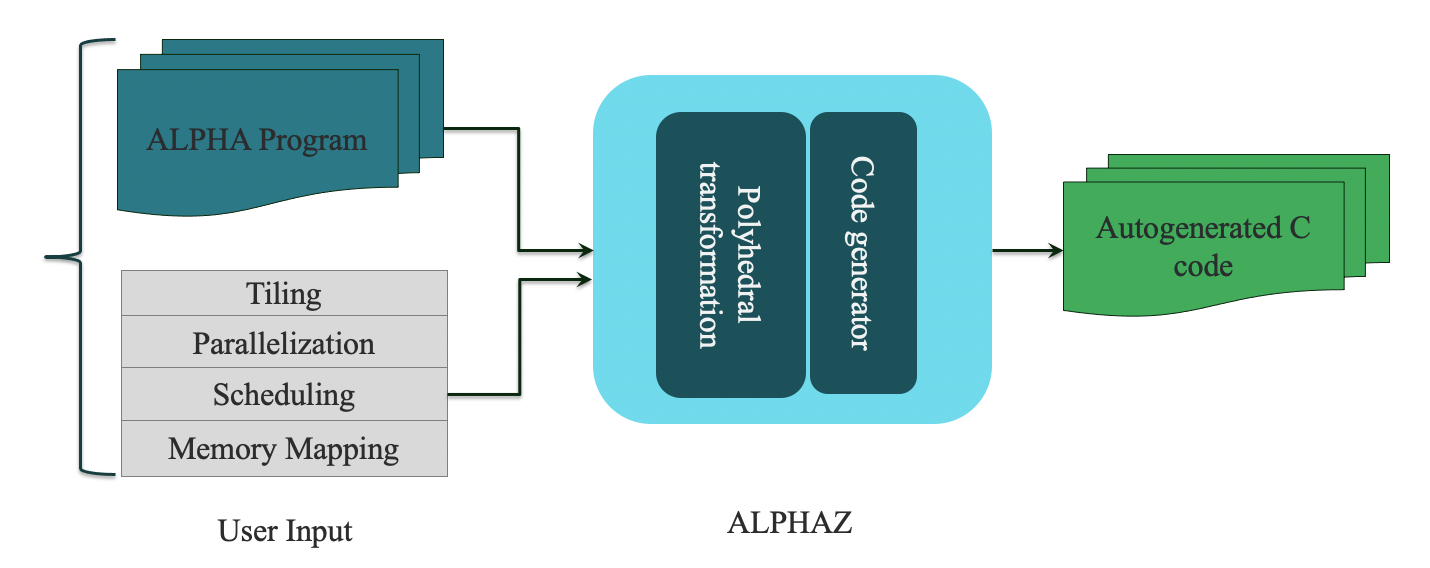
\includegraphics[scale=0.35,trim=5 5 5 5,clip]{content/figures/code_generation_methodology.png}}
\caption{Code generation methodology}
\label{fig:code_gen_methodlogy}
\end{figure}
\alphaz\ code optimization process has two parts – input specification and compilation script.  Input specification allows a user to express the computation using mathematical equations. The compilation script takes inputs (e.g., scheduling, parallelization, memory-mapping, and tiling transformations) from the user to generate optimized C code corresponding to the input specification. Figure~\ref{fig:code_gen_methodlogy} highlights the code optimization methodology using \alphaz\ .  


All the transformations in \alphaz\ are semantics preserving. However, it is the user's responsibility to ensure the transformations are valid. We use three important classes of transformations - target mappings, memory mappings, and tiling-related transformations. Target mappings-related transformations determine the execution order of the program. It allows the user to specify schedule and processor allocation for each variable in the system. It also allows the user to specify one or more dimensions of the schedule to be executed in parallel by different threads.  Memory mappings-related transformations allow multiple variables with different dimensions to share the same memory map based on the affine function. It also allows multiple variables with the same dimension to share memory space. Tiling transformations chop the iteration space to improve data locality and adjust parallelization granularity. Target and Memory mappings-related transformations require the user to specify the affine functions to indicate the schedule or memory map. The affine functions are expressed as $(ListOfIndices \mapsto ListOfIndexExpressions)$.
\begin{itemize}
    \item A schedule $(i, j \mapsto j, i)$ tells \alphaz\ that the iteration domain is $2$-dimensional represented by $i$, $j$ as the $ListOfIndices$, and the points in this iteration domain should be visited in the order given by the $ListOfIndexExpression$   $j$ and $i$.
    \item A memory map $(i, j \mapsto j, i)$ tells \alphaz\ that the mapping is associated with a $2$-D variable whose $(i, j)$-th element is stored at a location specified by $ListOfIndexExpressions$ - $(j, i)$.  It also allows the user to save memory if there is an opportunity for many-to-one mapping. E.g., $(i, j, k \mapsto i, j)$.
\end{itemize}

Efficient scheduled code generation depends on the choice of target and memory mappings-related transformations. 
Algorithm~\ref{algo:matrix_mul_alphabets} highlights the \alfa\ program for matrix multiplication. Algorithm~\ref{algo:matrix_mul_script} presents a compiling script for matrix multiplication that produces the C code highlighted in Listing~\ref{listing:alpha_code_gen}.


\begin{algorithm}
\caption{Matrix Multiplication in Alphabets}
\begin{algorithmic} [1]
\STATE \textbf{affine} MM $\lbrace N,K,M \mid (M, N, K)  > 0  \rbrace$
\STATE \textbf{input}
\STATE  \hspace{10pt} float A $\lbrace i, j \mid 0 \leq i < M \hspace{2pt} \&\& \hspace{2pt} 0 \leq j < K   \rbrace$ ;
\STATE  \hspace{10pt} float B $\lbrace i, j \mid 0 \leq i < K \hspace{2pt} \&\& \hspace{2pt} 0 \leq j < N   \rbrace$ ;
\STATE \textbf{output}
\STATE  \hspace{10pt} float C $\lbrace i, j \mid 0 \leq i < M \hspace{2pt} \&\& \hspace{2pt} 0 \leq j < N   \rbrace$;
\STATE \textbf{local}
\STATE \hspace{10pt} \slash \slash \text{local variables}
\STATE \textbf{output}
\STATE \hspace{10pt} C[$i,j$] = reduce(+, \hspace{2pt} [$k$], \hspace{2pt} A[$i,k$] * B[$k,j$]);
\end{algorithmic}
\label{algo:matrix_mul_alphabets}
\end{algorithm}
\begin{algorithm}
 \caption{Matrix Multiplication Command Script}
 \begin{algorithmic} [1]
 \STATE \text{\slash \slash \hspace{2pt}$Step-1: Parse \hspace{2pt} Alphabet \hspace{2pt} $}
 \STATE \text{prog=ReadAlphabets("MM.ab");}
 \STATE \text{system = “MM”;}
 \STATE \text{outDir="./src";}

 \STATE \text{}
 \STATE \text{\slash \slash \hspace{2pt}$Step-2: Perform \hspace{2pt} polyhedral \hspace{2pt}  transformation$}
 \STATE \text{Normalize(prog);}
 \STATE \text{setSpaceTimeMap(prog,  system,  “C”,  }
 \STATE \text{.  "($i,j,k \mapsto i, k, j$)", “($i,j \mapsto i, -1, j$)”); }
 \STATE \text{setParallel(prog,  system,  “”,  "0" );}
 \STATE \text{}
 \STATE \text{\slash \slash \hspace{2pt}$Step-3: Generate  \hspace{2pt} code$}
 \STATE \text{generateWriteC(prog,  system,  outDir);}
\STATE \text{generateScheduleC(prog,  system,  outDir);}
\end{algorithmic}
\label{algo:matrix_mul_script}
\end{algorithm}

\newpage
\begin{lstlisting}[label={listing:alpha_code_gen}, language=Caml, caption=Generated code - Matrix multiplication]
#define S1(i,j,i2) C(i,i2) = 0.0
#define S0(i0,i1,i2) C(i0,i2) = 
(C(i0,i2))+((A(i0,i1))*(B(i1,i2)))
{
    int c1,c2,c3;
    #pragma omp parallel for private(c2,c3)
    for(c1=0;c1 <= M-1;c1+=1){
	   for(c3=0;c3 <= N-1;c3+=1){
	       S1((c1),(-1),(c3));
	   }
       for(c2=0;c2 <= K-1;c2+=1){
            for(c3=0;c3 <= N-1;c3+=1){
                S0((c1),(c2),(c3));
            }
        }
    }
}

\end{lstlisting}


\textbf{Subsystems:} One of the primary challenges of using a polyhedral code generator is to produce readable, modular code. \alphaz\ subsystem construct is handy for addressing this. It helps organize a complex \alfa\ program into different parts capable of taking one or more \alfa\ variables as input to produce an output. \alphaz\ treats the subsystem itself like a variable to allow the user to specify a schedule for controlling the invocation and a memory map for optimizing variable passing between subsystem caller and callee. The subsystem invocations can be precisely controlled for any point in the iteration space.




